%\documentclass{beamer}
\documentclass[aspectratio=169]{beamer}
\usepackage{pgfpages}
% \setbeameroption{hide notes} % Only slides
% \setbeameroption{show only notes} % Only notes
\setbeameroption{show notes on second screen=right} % Both
\setbeamertemplate{note
page}{\pagecolor{yellow!8}\insertnote}\usepackage{palatino}
% page
% https://gist.github.com/andrejbauer/ac361549ac2186be0cdb

% \usetheme[hideothersubsections]{WrightState}
\usetheme[left,hideothersubsections,width=2cm]{WrightState} %2.5cm

\title{Data Mining Techniques and Mathematical Models for
the Optimal Scholarship Allocation Problem for a State University}
\author{Shuai Wang} %
\institute{Wright State University \\

	Department of Biomedical, Industrial, and Human Factors Engineering}
\date{December 6th, 2017}

\usepackage{natbib}  % for citation
\usepackage{comment}
\usepackage{geometry,array,graphicx,float,caption,subcaption,epstopdf,multiro
w}

% \usepackage{floatrow}
% \newfloatcommand{capbtabbox}{table}[][\FBwidth]

%https://tex.stackexchange.com/questions/193975/highlight-only-current
%-subsection-hide-subsections-of-other-sections

%https://tex.stackexchange.com/questions/193975/highlight-only-current
%-subsection-hide-subsections-of-other-sections

\setcounter{tocdepth}{1} % hide subsection in the table of content

\AtBeginSection[]{
% \ifnum \value{framenumber}>1
\begin{frame}<beamer>
%    \frametitle{Outline for section \thesection}
    \tableofcontents[currentsection]
  \end{frame}
}


\begin{comment}
\makeatletter
  \setbeamertemplate{sidebar \beamer@sidebarside}%{sidebar theme}
  {
    \beamer@tempdim=\beamer@sidebarwidth%
    \advance\beamer@tempdim by -6pt%
    \insertverticalnavigation{\beamer@sidebarwidth}%
    \vfill
    \ifx\beamer@sidebarside\beamer@lefttext%
    \else%
      \usebeamercolor{normal text}%
      \llap{\usebeamertemplate***{navigation symbols}\hskip0.1cm}%
      \vskip2pt%
    \fi%
}%
\makeatother
\end{comment}

% ------ begin ---------------------------------------

\begin{document}

%{% open a Local TeX Group
% \setbeamertemplate{sidebar}{}
\begin{frame}
        \titlepage
       
     \note[item]{Thank for attending my thesis defense.}
      \note[item]{My name is Shuai Wang, and I am from BIE department}
\note[item]{my thesis title is Data Mining Techniques and Mathematical Models
for the Optimal Scholarship Allocation Problem for a State University}
\note[item]{essentially, i am trying to study what is the ideal scholarship for
each individual and what is the optimal schohapship budget for school}
\end{frame}
%}% end Local TeX Group


\begin{frame}
    \frametitle{Presentation Outline}
    
 \tableofcontents
 \note[item]{Here is the outline of my presentation}
\end{frame}


\section{Introduction}  

\subsection{Background}
\begin{frame}
    \frametitle{Background}
\begin{itemize}
\item In the United States, the 2012-2013 academic year, there were a total 
of 20.4 million students in degree-granting institutions.
\item More than 80\% of them received financial aid.

\item Studies have shown that financial aid is one of the most important
factors in attracting student and is vital to enrollment management.
\end{itemize}
\note[item]{first,I'd like to talk about the background of the study}
\note[item]{From the latest department of education report}
%\note[item]{Grant are usually are need-based}
\end{frame}

\begin{frame}
	\frametitle{Background Cont.}
    Enrollment management consisted of approaches to help university
to meet the established goal such as:
   \begin{itemize}
   \item Attract more high-caliber students.
   \item Diversify student body.
   \item Increase retention.
   \item Improve graduation rate.
   \end{itemize} 

\end{frame}



\begin{frame}
\frametitle{Scholarship}
\begin{itemize}
  \item Scholarship is the focused type of financial aid of the study.
  \item Scholarship is the major marketing tool for targeting students.
  \item Scholarship helps the university:
\begin{enumerate}
\item Giving more access to families who need help.
\item Stimulating more students to major in area having labor shortage.
\item Diversifying the student body.
\end{enumerate}
\item Merit-based scholarship.
\end{itemize}


\note[item]{LAST: For example, some schools offer targeted scholarship for
minorities students}
\note[item]{ There are various types of scholarships, For this 
study, we only focus on merit-based scholarship, which means, we only consider
applicant's academic performance}

\end{frame}



\subsection{Motivation}
\begin{frame}
\frametitle{Motivation}

\begin{enumerate}
\item \textbf{Non-optimal} usage of scholarship budget at 
    university: 

\begin{itemize}
\item   Over-spending scholarship budget would reduce revenue.
\item   Under-spending scholarship would potentially
undermine enrollment number and revenue. 
\end{itemize}

\item The tuition income accounts for 48\% of the 
yearly revenue of the university under study.

\item The optimal allocation of scholarship problem has 
\textbf{not} been widely studied in literatures.

\end{enumerate}
\note[item]{Here is the motivation of the study}
\note[item]{First let's see what happens if the school
does not use the scholarship budget properly.}
\note[item]{There two kinds of improper usage of scholarship, the first one is
the second of is, they both could porentially reduce the revene and
under-spending could also undermine the enrollment number}
\end{frame}




\subsection{Research Questions and Contribution}
\begin{frame}  
    \frametitle{Research Questions and Contribution}
\begin{itemize}
  \item Research questions:
   \begin{enumerate}
    \item How does scholarship affect student's
    decision?
\item What is the optimal scholarship for each student under the 
    overall budget?
\item What is the ideal scholarship budget for school?
\end{enumerate}


\item Contribution: 

Utilized various data mining and optimization techniques to solve the above
questions.
\end{itemize}

\note[item]{Here comes the reseach questions I want to answer in the study}

\end{frame}


%%%%%%%%%%%%%%%%%%%%%%







\subsection{Results Example}
\begin{frame}
    \frametitle{Results example}
    
    
Enrollment probability of students with various background under different
scholarship level.
   
\begin{table}[H]
\centering
 % \tiny 43
 \scriptsize % 169
 \setlength\tabcolsep{3pt}
    \begin{tabular}{|c|c|c|c|c|c|c|c|c|c|c|}
    \hline %\hline
    \multicolumn{11}{ |c| }{GPA 2.9, ACT 19 }  \\ \hline
& Student               & 0       & 1000    & 2000    & 3000    & 4000    &5000
& 6000    & 7000    & 8000       \\ \hline
1& 2.9-Tier1-19-White    & 59.55 & 64.63 & 69.39 & 73.77 & 77.73 & 81.24 &
84.31 & 86.96 & 89.22  \\ \hline

2& 2.9-Tier5-19-White    & 36.96 & 40.20 & 43.53 & 46.92 & 50.34 & 53.75 &
57.13 & 60.45 & 63.67  \\ \hline
     \multicolumn{11}{ |c| }{GPA 3.3, ACT  25 }   \\ \hline
3& 3.3-Tier1-25-Hispanic & 23.80 & 27.44 & 31.42 & 35.69 & 40.20 & 44.88 &
49.65 & 54.43 & 59.13  \\ \hline
4& 3.3-Tier1-25-White    & 55.60 & 59.32 & 62.94 & 66.42 & 69.72 & 72.84 &75.75
& 78.43 & 80.90  \\ \hline
    \multicolumn{11}{ |c| }{GPA 3.8, ACT 28 }     \\ \hline
5& 3.8-Tier1-28-White    & 42.29 & 46.05 & 49.85 & 53.65 & 57.41 & 61.08 &64.63
& 68.03 & 71.25  \\ \hline
6& 3.8-Tier4-28-White    & 20.54 & 22.87 & 25.37 & 28.05 & 30.89 & 33.89 &37.02
& 40.26 & 43.60  \\ \hline
    \end{tabular}
    \end{table}



\note[item]{Here are results of students' reaction to various amount of 
scholarship  offered}
\note[item]{2.9 Tier1 19 white means a student have GPA 2.9, from 
Tier1, 19 ACT, white}
\note[item]{We can see the probability of enrollment of this student 
    is increasing
with money offered.}
\note[item]{I will explain more about the table later in the methodology
section}
\end{frame}






\begin{frame}
\frametitle{Results example}
Using prediction of enrollment, graduation and number of years as input,
and the optimization model yields:

\begin{figure}[ht]
    \centering
    \includegraphics<1>[width=4in, height=2in,scale=0.2]{pic/ssi_14k.eps} 
    \end{figure}     
\note[item]{By using the prediction of enrollment, graduation and number of
years as INPUT of the optimization mode the results look like this:}
\note[item]{in the begining , the objective which is revenue increased with 
the incerease of budget, and reach to the highest at when 2.8 million}
 

\note[item]{When SSI= 14000, the total revenue increase increase when
     more budget are used , then reaches to the highest revenue at about 2.8
     million, and start to decrease when budget increases,
     
     
     
          so 2.8 million is the sweet spot here
}
     
     

\end{frame}
	
	



\begin{frame}
\frametitle{Results example}
\begin{figure}
	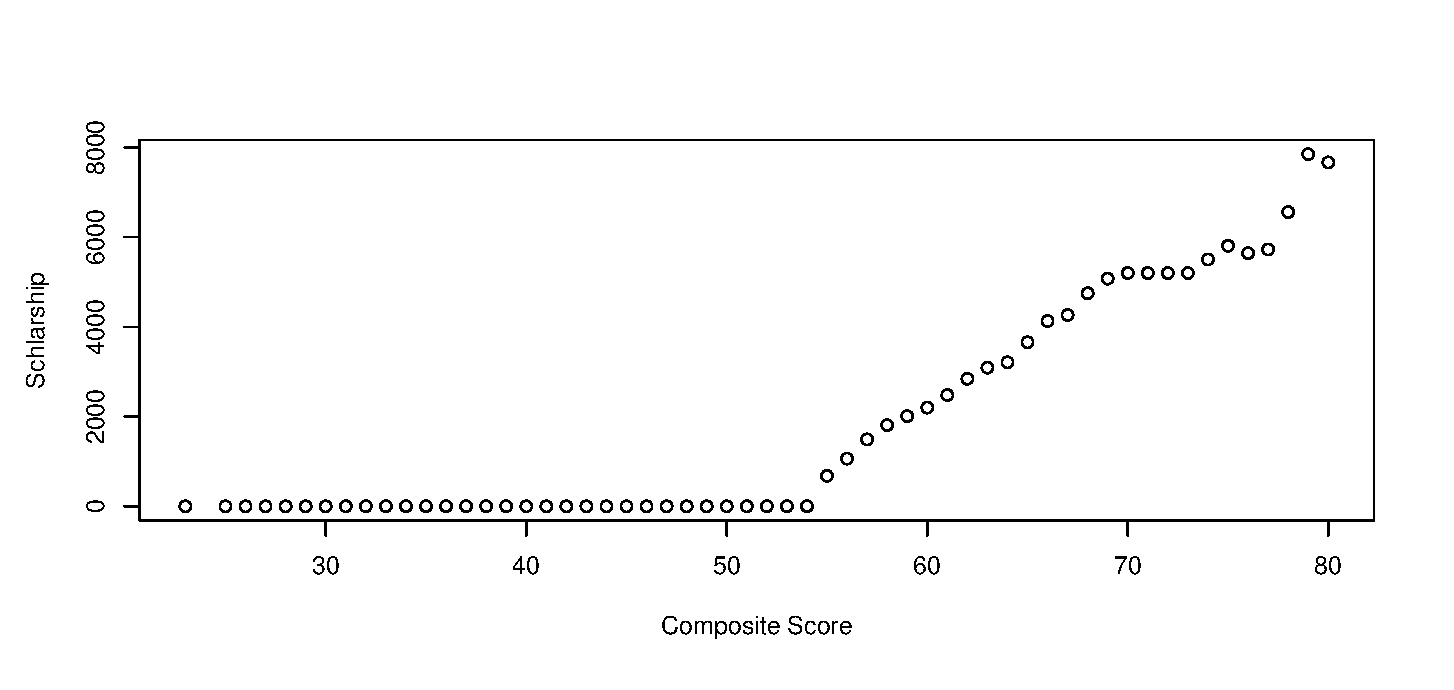
\includegraphics[width=4in,height=2in,scale=0.4]{pic/scho_composite.eps}
    
    Average scholarship allocation  vs combine score when SSI=14,000
\note[item]{this graph shows the optimization results when ssi=14,000 against 
composite schore}
    \note[item]{The scholarship increases along with the increase of the
composite score}
\end{figure}

\end{frame}







%-----------liter review---------------------
\section{Literature Review}
\subsection{Student Demand Model at Macro-level}


\begin{frame}
  \frametitle{Macro and micro level of enrollment study}
  Traditional enrollment studies:
  \begin{itemize}
    \item Macro level student demand studies.
    \item Micro level students college choice models.
  \end{itemize}
  
  \note{Before we dive into the fancy prediction and optimization model,
  let's first look at what have been done in the
literature in the realated fields such as Macro level student demand studies
and micro level
students college choice modes to understand  the underlying factors which are
going to be used later in the prediction and optimization model.}
  
\end{frame}

\begin{frame}
  \frametitle{Macro level student demand studies}
  Impact of the increasing tuition on enrollment decisions.
  
  Questions include \citep{Leslie1987,  Leslie1988, Heller1997,
                          Ehrenberg2004, Crouse2015}:
  
 \begin{itemize}
   \item What happens to the enrollment when universities raise 
   their tuition?
  \item What is the net impact of higher tuition and reduced enrollment 
  upon institutional finance?
  \item Who will not attend university because of the increasing tuition?


 \end{itemize}
 
  \note[item]{The macro level student demand theroy studies what is the impact
of the increasing tuition on the student's enrollment decision}
\end{frame}

\begin{frame}
    \frametitle{Macro level student demand studies}

\begin{itemize}
  \item The increasing tuition leads to reduction in enrollment:
  
%\begin{enumerate}
%\item What are the impact of revenue and enrollment number if the tuition
%increases? 
%\end{enumerate}


\begin{enumerate}
  \item \citet{Leslie1987} found that every \$100 tuition increase came 
  with a 0.7\% drop in enrollment.
\item \citet{Crouse2015} found a \$100 
increase in tuition would lead to a decline in enrollment of about 0.88\%. 

\end{enumerate}


\end{itemize}

\note[item]{And studies found that  higher tuition prices.....}
\end{frame}


\begin{frame}
  \frametitle{Macro level student demand studies}
    However:
  \begin{itemize}
    \item  Tuition kept increasing in the past decades.
    \item Enrollment still grows.
    
  \end{itemize}
  
 Ameliorating effects of financial aid \citep{Leslie1987}.
  
\end{frame}



\begin{frame}
    \frametitle{Macro level student demand studies}
 Student demand theory on financial aid:
 
How does student response to the changes of financial aid.
\begin{itemize}
\item  \citet{Braunstein1999} found that every \$1,000 increase in
financial aid, the probability of enrollment increased between 1.1\% and
2.5\%.

 \end{itemize}
 
 \end{frame}




\begin{frame}
    \frametitle{Targeting Effect of Financial Aid on Students 
    with Various Characteristics}

Targeting effects of financial aid vs broader effects of tuition.

\begin{enumerate}
  \item The following group of students are more sensitive to 
  changes of tuition:

 \begin{itemize}
 \item Low income students \citep{Crouse2015}.
 \item  African American and Latino students \citep{Hossler1989}.
 \end{itemize}
 
\item High-caliber students are less sensitive to
 the increase of tuition \citep{Heller1999}.

\end{enumerate}

\note[item]{ we all  know that all students  are affected by  the 
tuition increase,  but it is important to understand students with
different background can react differently to changes in financial aid.
Studies found that}

\note[item]{One reason is that high-caliber students have more scholarship
offer}

\end{frame}





\begin{frame}
  \frametitle{Micro level student choice model}
  \begin{itemize}
    \item Student demand studies, at macro level, investigates the 
    enrollment decisions associated with \textbf{groups} of students.
    \item Student choice model, at micro level, studies the individual
student's decision to enrollment at particular university.
  \end{itemize}
  
 \note[item]{Previously, I talked about the student demand studies, it
investigates how does a group of student react to the changes in tuition and
finacial aid}

\note[item]{in order to understand what impact student's decision at 
individual level, the sudent choice model are studied}
  \end{frame}


\subsection{Enrollment Prediction at Micro Level}
\begin{frame}
    \frametitle{Enrollment Prediction at Micro Level}
    \begin{enumerate}
    \item Predicting individual student's enrollment decision.
    
    \item Type of variables used in the prediction model:
\citet{Paulsen1990,Hossler1998}:
    \begin{itemize}
    \item Academic (GPA, ACT/SAT, Percentile)
    \item Financial (Income, Pell Grant, etc,.)
    \item Demographic (Ethnicity, First language, 
    High school, Home distance to campus, etc,.)
    \end{itemize}
    \end{enumerate}
    
  \note[item]{The outcome of decision model is binary 0 or 1, enrolled or not,
graduated or not}
\end{frame}

\begin{frame}
    \frametitle{Response to Financial Aid and Optimization at Micro 
    Level}
    Objective of the mathematic modeling in the literature:
    \begin{enumerate}
    \item Maximize index: SAT
      \citep{Ehrenberg1984,Sugrue2010}.
    \item Maximize tuition revenue \citep{Thanh2007}.
    \end{enumerate}
    
   \note[item]{There are only few literature using the optimization
techniques.}
   \note[item] {The first one is to maximize the number of student 
   within a certain SAT range}
   \note[item]{the second one is to achieve a better SAT score as 
   possible while maintaining the same amount students}
   
\end{frame}

\begin{frame}
    \frametitle{Response to Financial Aid and Optimization at Micro Level}
    Constraints of the mathematic modeling in the literature:
    \begin{enumerate}
    \item Capacity and faculty-student ratio
    \citep{Thanh2007}.
    
    \item Availability of students in expected SAT range, 
    budget, and capacity
    \citep{Sugrue2010}.
    
    \end{enumerate}
    \note[item]{capacity can be under school, college, and department level}
\end{frame}


\begin{frame}
   \frametitle{Response to Financial Aid and Optimization at Micro Level}
 
 Issues of these studies:
 
 \begin{enumerate}
\item Did not address the allocation of financial aid for students with 
various socioeconomic characteristics.
\item Did not address how to optimally allocate scholarship at the
aggregate level.
 \end{enumerate}

\end{frame}


\section{Methodology and Results}


\begin{frame}
\frametitle{Objective of the optimization model}
\begin{itemize}
  \item   Objective of the optimization model: 
  Revenue income + SSI income
 \item Revenue income:
  Prob E * (Tuition - Scholarship)* NumYears

\item SSI income:
  Prob E * Prob G * SSI
\end{itemize}

\note[item]{i want to talk about objective of the optimization model first,
because it links all the rest components together}
\end{frame}





\subsection{Enrollment and Graduation Prediction}
\begin{frame}
    \frametitle{Enrollment and graduation outcome prediction}
    \begin{itemize}
      \item The outcome of enrollment and graduation problem is binary (yes or
no). 
\item It is a two-class classification problem.
\item  Common methods for two-class classification problem:

logistic regression, decision tree, svm, etc,.
    \end{itemize}



\note[item]{START: Let's see the how to predict enrollment and graduation}
\end{frame}

\begin{frame}
\frametitle{Logistic Regression}
Logistic regression was used as the base line model.

Why linear regression does not work?
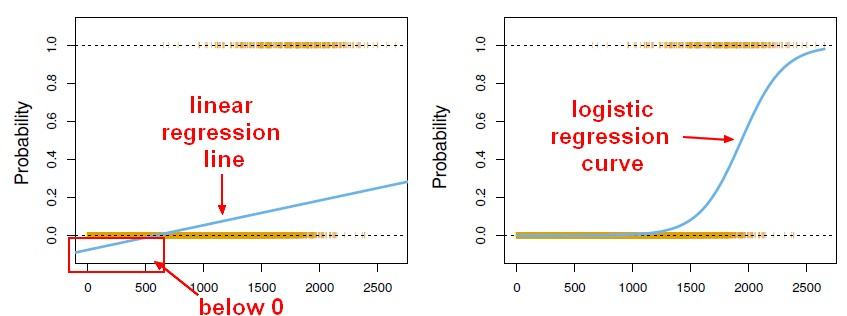
\includegraphics[scale=0.345]{pic/logistic_regression_vs_linear.jpg}
\note[item]{The linear regression model is based on an assumption that 
the outcome Y is continuous, with errors are normally distributed.}
\note[item]{if the outcome is binary, this is clearly violated}
\note[item]{Predicted values may be out of range, for 0,1, the linear
regression prediction will be out of this range.

So we need to find a type of regression which can predict the value from 0-1}
\end{frame}

\begin{frame}
    \frametitle{Logistic Regression}


The goal of logistic regression is to find:

\begin{itemize}
\item Best fitting  model to describe the relationship between the 
binary outcome and a set of independent variables. 
\end{itemize}

\end{frame}





\begin{frame}
\frametitle{Logistic Regression: Variables}

\begin{enumerate}
\item Academic: HS GPA, ACT/SAT, HS Percentile.
\item Financial: Pell Grant, EFC, Out-of-pocket, Scholarship,
	Unemployment rate.
\item Demographic: High School, Tier, Ethnicity. 
    
\end{enumerate}

\end{frame}



\begin{frame}
\frametitle{Logistic Regression: Enrollment prediction results}
\begin{table}[H]
\centering
 % \tiny 43
 \scriptsize % 169
 \setlength\tabcolsep{3pt}
    \begin{tabular}{|c|c|c|c|c|c|c|c|c|c|c|}
    \hline %\hline
    \multicolumn{11}{ |c| }{GPA 2.9, ACT 19 }  \\ \hline
& Student               & 0       & 1000    & 2000    & 3000    & 4000    &5000
& 6000    & 7000    & 8000       \\ \hline
1& 2.9-Tier1-19-White    & 59.55 & 64.63 & 69.39 & 73.77 & 77.73 & 81.24 &
84.31 & 86.96 & 89.22  \\ \hline

2& 2.9-Tier5-19-White    & 36.96 & 40.20 & 43.53 & 46.92 & 50.34 & 53.75 &
57.13 & 60.45 & 63.67  \\ \hline
     \multicolumn{11}{ |c| }{GPA 3.3, ACT  25 }   \\ \hline
3& 3.3-Tier1-25-Hispanic & 23.80 & 27.44 & 31.42 & 35.69 & 40.20 & 44.88 &
49.65 & 54.43 & 59.13  \\ \hline
4& 3.3-Tier1-25-White    & 55.60 & 59.32 & 62.94 & 66.42 & 69.72 & 72.84 &75.75
& 78.43 & 80.90  \\ \hline
    \multicolumn{11}{ |c| }{GPA 3.8, ACT 28 }     \\ \hline
5& 3.8-Tier1-28-White    & 42.29 & 46.05 & 49.85 & 53.65 & 57.41 & 61.08 &64.63
& 68.03 & 71.25  \\ \hline
6& 3.8-Tier4-28-White    & 20.54 & 22.87 & 25.37 & 28.05 & 30.89 & 33.89 &37.02
& 40.26 & 43.60  \\ \hline
    \end{tabular}
\end{table}


\note{ The prediction of graduation has the same fashion
}

\end{frame}

\subsection{Number of Years Prediction}

\begin{frame}
\frametitle{Number of years prediction}

\begin{itemize}
  \item It is a regression problem.
  \item The following methods are compared to predict the years of stay in
school:

\begin{table}[H]
\centering
%\scriptsize
\small
\label{num_year}
\begin{tabular}{|c|c|c|c|c|} \hline
    & \multicolumn{2}{c|}{10-Fold Cross Validation} &
\multicolumn{2}{c|}{Test Data} \\ \hline
Model                        & RMSE                  & MAE                   &
RMSE           & MAE           \\ \hline
GLM                          & 1.40                  & 1.2                   &
1.53           & 1.26          \\ \hline
SVM (Linear Kernel)           & 1.44                  & 1.20                  &
1.62           & 1.32          \\ \hline
Decision Tree                         & 1.43                  & 1.24        &
1.43           & 1.23          \\ \hline
Stochastic Gradient Boosting & 1.40                  & 1.19                  &
\textbf{1.40}           & \textbf{1.19}    \\
\hline
\end{tabular}
\end{table}

\end{itemize}

\note[item]{A gradient descent procedure is used to minimize the loss when
adding trees. weaker learner to better learner}
\end{frame}


\subsection{Optimization Model}
\begin{frame}
\frametitle{Why prediction model is not enough?}
\begin{enumerate}
  \item The prediction of enrollment and graduation provide some 
insights of how students response to the various scholarship. 
  \item They have not addressed the allocation of limited
scholarship budget to students fundamentally.

\note[item]{ most literatures end up in the phase 1 to predict the enrollment,
 and tells you what factors are important but there is not further
action}

\note[item]{And in this study, we are trying to solve this by using
optimization model, which is main contribution of thesis}
\end{enumerate}


% Questions like the following are addressed: 
% \begin{enumerate}
% \item Should we allocate the money to local students as they 
% are our bread and butter students and require less money?
% \item Should we allocate the money to 
% far-away students as local students will come anyway?
% \end{enumerate}  
\end{frame}


\begin{frame}
\frametitle{Objective Model}
\textbf{Sets}:
\begin{itemize}
\item I:   set of applicants,  indexed by $i$ and $j$ \\
\item  M:  different levels of scholarship awards, indexed by 
$m$\\
$m \in  M = \{ 0,1000, 2000, \ldots ,8000\} $ \end{itemize}


\textbf{Variables}:
\begin{itemize}
\item $x_{im}$ :
binary, whether a scholarship award $m$ is allocated to applicant $i$ or not
\end{itemize}

\end{frame}

\begin{frame}
\frametitle{Math notation}

\textbf{Parameters}:
\begin{itemize}
\item $p^e_{im}$: \hspace{0.3cm}  probability of enrollment for applicant 
$i$, if given award $m$
\item $p^g_{im}$: \hspace{0.3cm}  probability of graduation for applicant 
$i$, if given award $m$ 
\item $N_{im}$: \hspace{0.25cm} expected number of years student $i$ 
stays at the institution, if given award $m$
\item $d(i,j)$:\hspace{0.1cm} 1 if applicant $i$ dominates 
applicant $j$; 0 otherwise
\item B:       \hspace{0.3cm} total budget for financial aid
\item $A_m$: \hspace{0.01cm} monetary value of award $m$
\item $T_i$:  \hspace{0.2cm} tuition paid by applicant $i$
\item $SSI_i$:\hspace{0cm} government compensation for
				applicant $i$ graduates

\end{itemize}
\end{frame}




\begin{frame}{fragile}
\frametitle{Objective}
\textbf{Maximize the total revenue}: Tuition revenue + SSI 
income:

\scriptsize{
$\max \quad \sum_{i\in I} \sum_{m\in M} x_{im}\cdot p^e_{im}\cdot(T_i-A_m)\cdot
N_{im}+
\sum_{i\in I} \sum_{m\in M} x_{im}\cdot p^e_{im} \cdot p^g_{im}\cdot SSI_i$

}


\end{frame}


\begin{frame}
\frametitle{Constraints}
\begin{enumerate}
\item Each student only gets one scholarship:

 $\sum_{m \in 
M}x_{im}=1  \hspace{0.5cm} \forall i\in I $
\vfill
\item Total budget constraint: 

$\sum_{i \in I} \sum_{m\in M} 
x_{im}\cdot p^e_{im}\cdot A_m\leq B $
\vfill
\item Dominance constraint:

$ \sum_{m \in M} x_{im}\cdot A_m \geq \sum_{m \in M} 
x_{jm}\cdot A_m \hspace{0.5cm}  \forall
(i,j)|d(i,j)=1 $

\end{enumerate}
\end{frame}



\begin{frame}
\frametitle{Pair-wise Dominance Constraints}
Around 5,500 applicants each year.

For the dominance constraints:

There are $(5,500 \times 5,500) / 2$ or 
more than 15 million constraints.

\begin{table}[H]
\centering
\begin{tabular}{|c|c|c|}
\hline
  Applicant & GPA & ACT \\ [0.5ex] 
\hline
1 & 2.9 & 18 \\ \hline
2 & 3.7 & 21 \\ \hline
3 & 3.8 & 30 \\ \hline
4 & 2.7 & 21 \\ \hline
5 & 3.3 & 17 \\ \hline
6 & 3.9 & 27 \\ \hline
\end{tabular}

\note{there are about 55 hundred applicants each year}
\note{15 millions constraints is very hard to solve using the standard solver,
so this should be reduced } 
\end{table}

\end{frame}

\begin{frame}
\frametitle{Full and redundant dominance }

 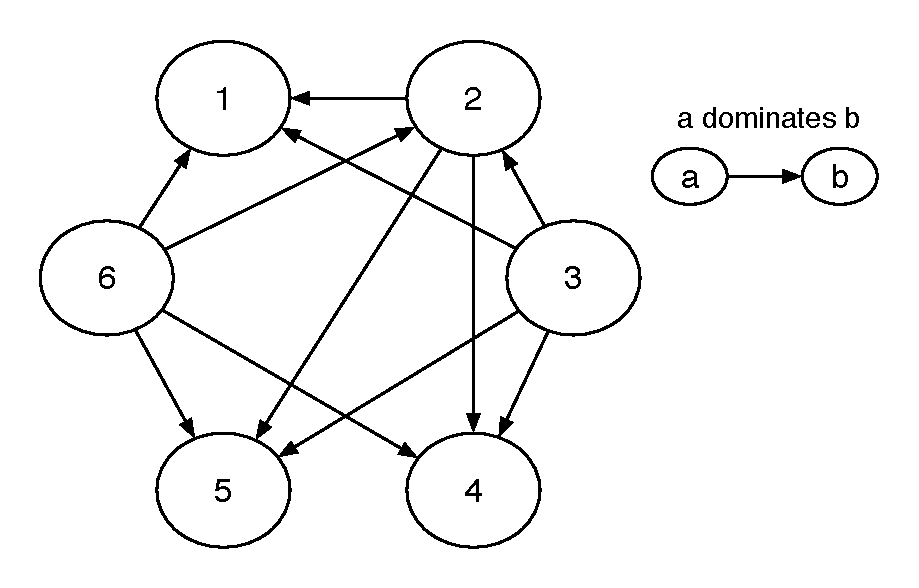
\includegraphics[scale=0.5]{pic/dominance1.eps}
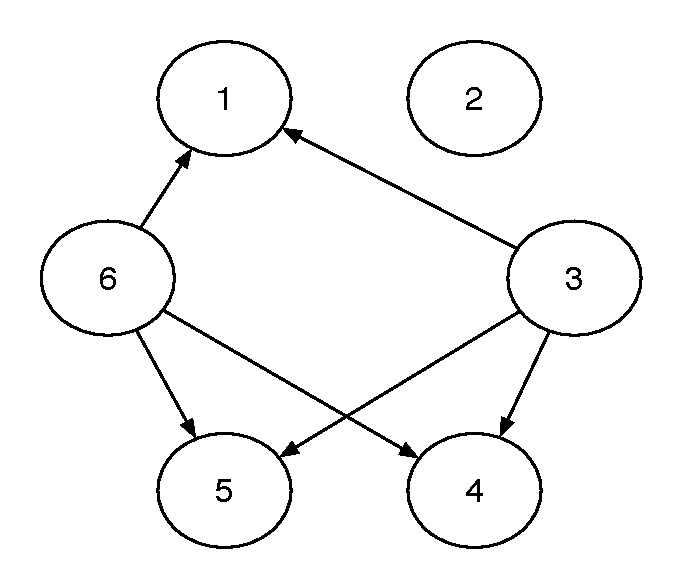
\includegraphics[scale = 0.5]{pic/dominance2.eps}

$ \sum_{m \in M} x_{im}\cdot A_m \geq \sum_{m \in M} 
x_{jm}\cdot A_m \hspace{0.5cm}  \forall
(i,j)|d(i,j)=1 $

There are total 11 constraints in this case, 6 of them are redundant.

\end{frame}

\begin{frame}
\frametitle{Minimum dominance}
\begin{center}
 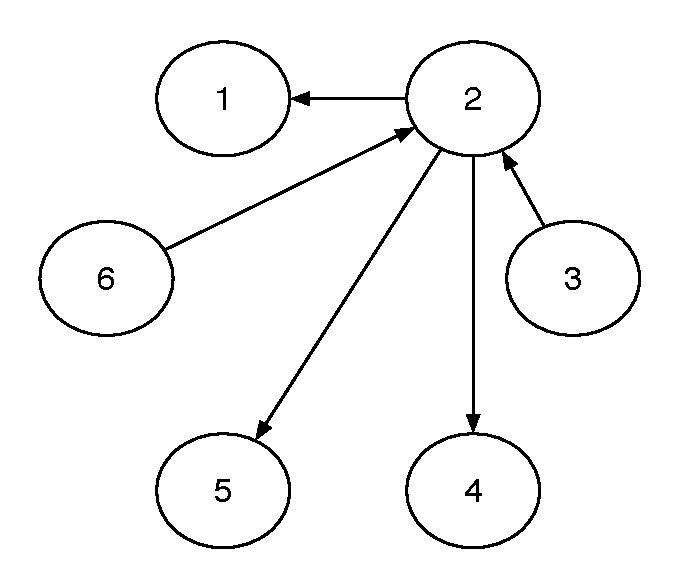
\includegraphics[scale = 0.35]{pic/dominance3.eps}
\end{center}
 
 \small{
\begin{center}
 \begin{tabular}{l|llllll}
        & 1 & 2 & 3 & 4 & 5 & 6 \\ \hline
        1 & 0 & 0 & 0 & 0 & 0 & 0 \\
        2 & 1 & 0 & 0 & 1 & 1 & 0 \\
        3 & 0 & 1 & 0 & 0 & 0 & 0 \\
        4 & 0 & 0 & 0 & 0 & 0 & 0 \\
        5 & 0 & 0 & 0 & 0 & 0 & 0 \\
        6 & 0 & 1 & 0 & 0 & 0 & 0
    \end{tabular}
\end{center}
    }
\end{frame}


\begin{frame}
\frametitle{Size of the optimization models}

\centering
\small{
\begin{tabular}{|c|l|c|c|}
\hline %\hline
\multicolumn{2}{|c|}{Model Components}   &
Original Model & Reduced Model \\ \hline
Variables                   & \multicolumn{1}{|l|}{Allocation (binary) 
$x_i$}
& 57,860         & 57,860        \\ \hline
\multirow{3}{*}{Constraint} & One Award per ID         &
5,260          & 5,260         \\ \cline{2-4}
& Dominance                & \textbf{13,833,800}    & \textbf{191,497}
\\ \cline{2-4}
& Total Budget              & 1              & 1
\\ \cline{2-4}
& Total Number of Constraints     & 13,839,061     & 196,758
\\ \hline
\end{tabular}
}


\end{frame}



%\begin{frame}
%\frametitle{Optimization Results}
%\begin{figure}
%    \centering
%  \includegraphics[width=8cm, height=6cm,scale=0.2]{pic/ssi_10k.eps}
%\end{figure}
%\end{frame}
%
%
%\begin{frame}
%\frametitle{Optimization Results}
%\begin{figure}
%    \centering
%  \includegraphics[width=8cm, height=6cm,scale=0.2]{pic/ssi_12k.eps}
%\end{figure}
%\end{frame}


\begin{frame}
\frametitle{Optimization Results}
\begin{figure}
    \centering
  \includegraphics[width=8cm, height=6cm,scale=0.2]{pic/ssi_14k.eps}
\end{figure}


\note{As we see from the graph, 2.8 million yields the best objective,
bugget lower than 2.8 million is underspending and greater than 2.8 million
is overspending.}
\end{frame}

\subsection{Implementation}

\begin{frame}
\frametitle{Policy and Implementation}
\begin{itemize}
\item First phase solves the prediction problems.
\item Second phase solves optimal allocation problem.
\item Enrollment administration needs a 
simple policy to implement.
\item  Decision tree and piecewise linear regression were used for this task.
\end{itemize}
 
\end{frame}

\begin{frame}
\frametitle{Decision tree policy}
\begin{center}
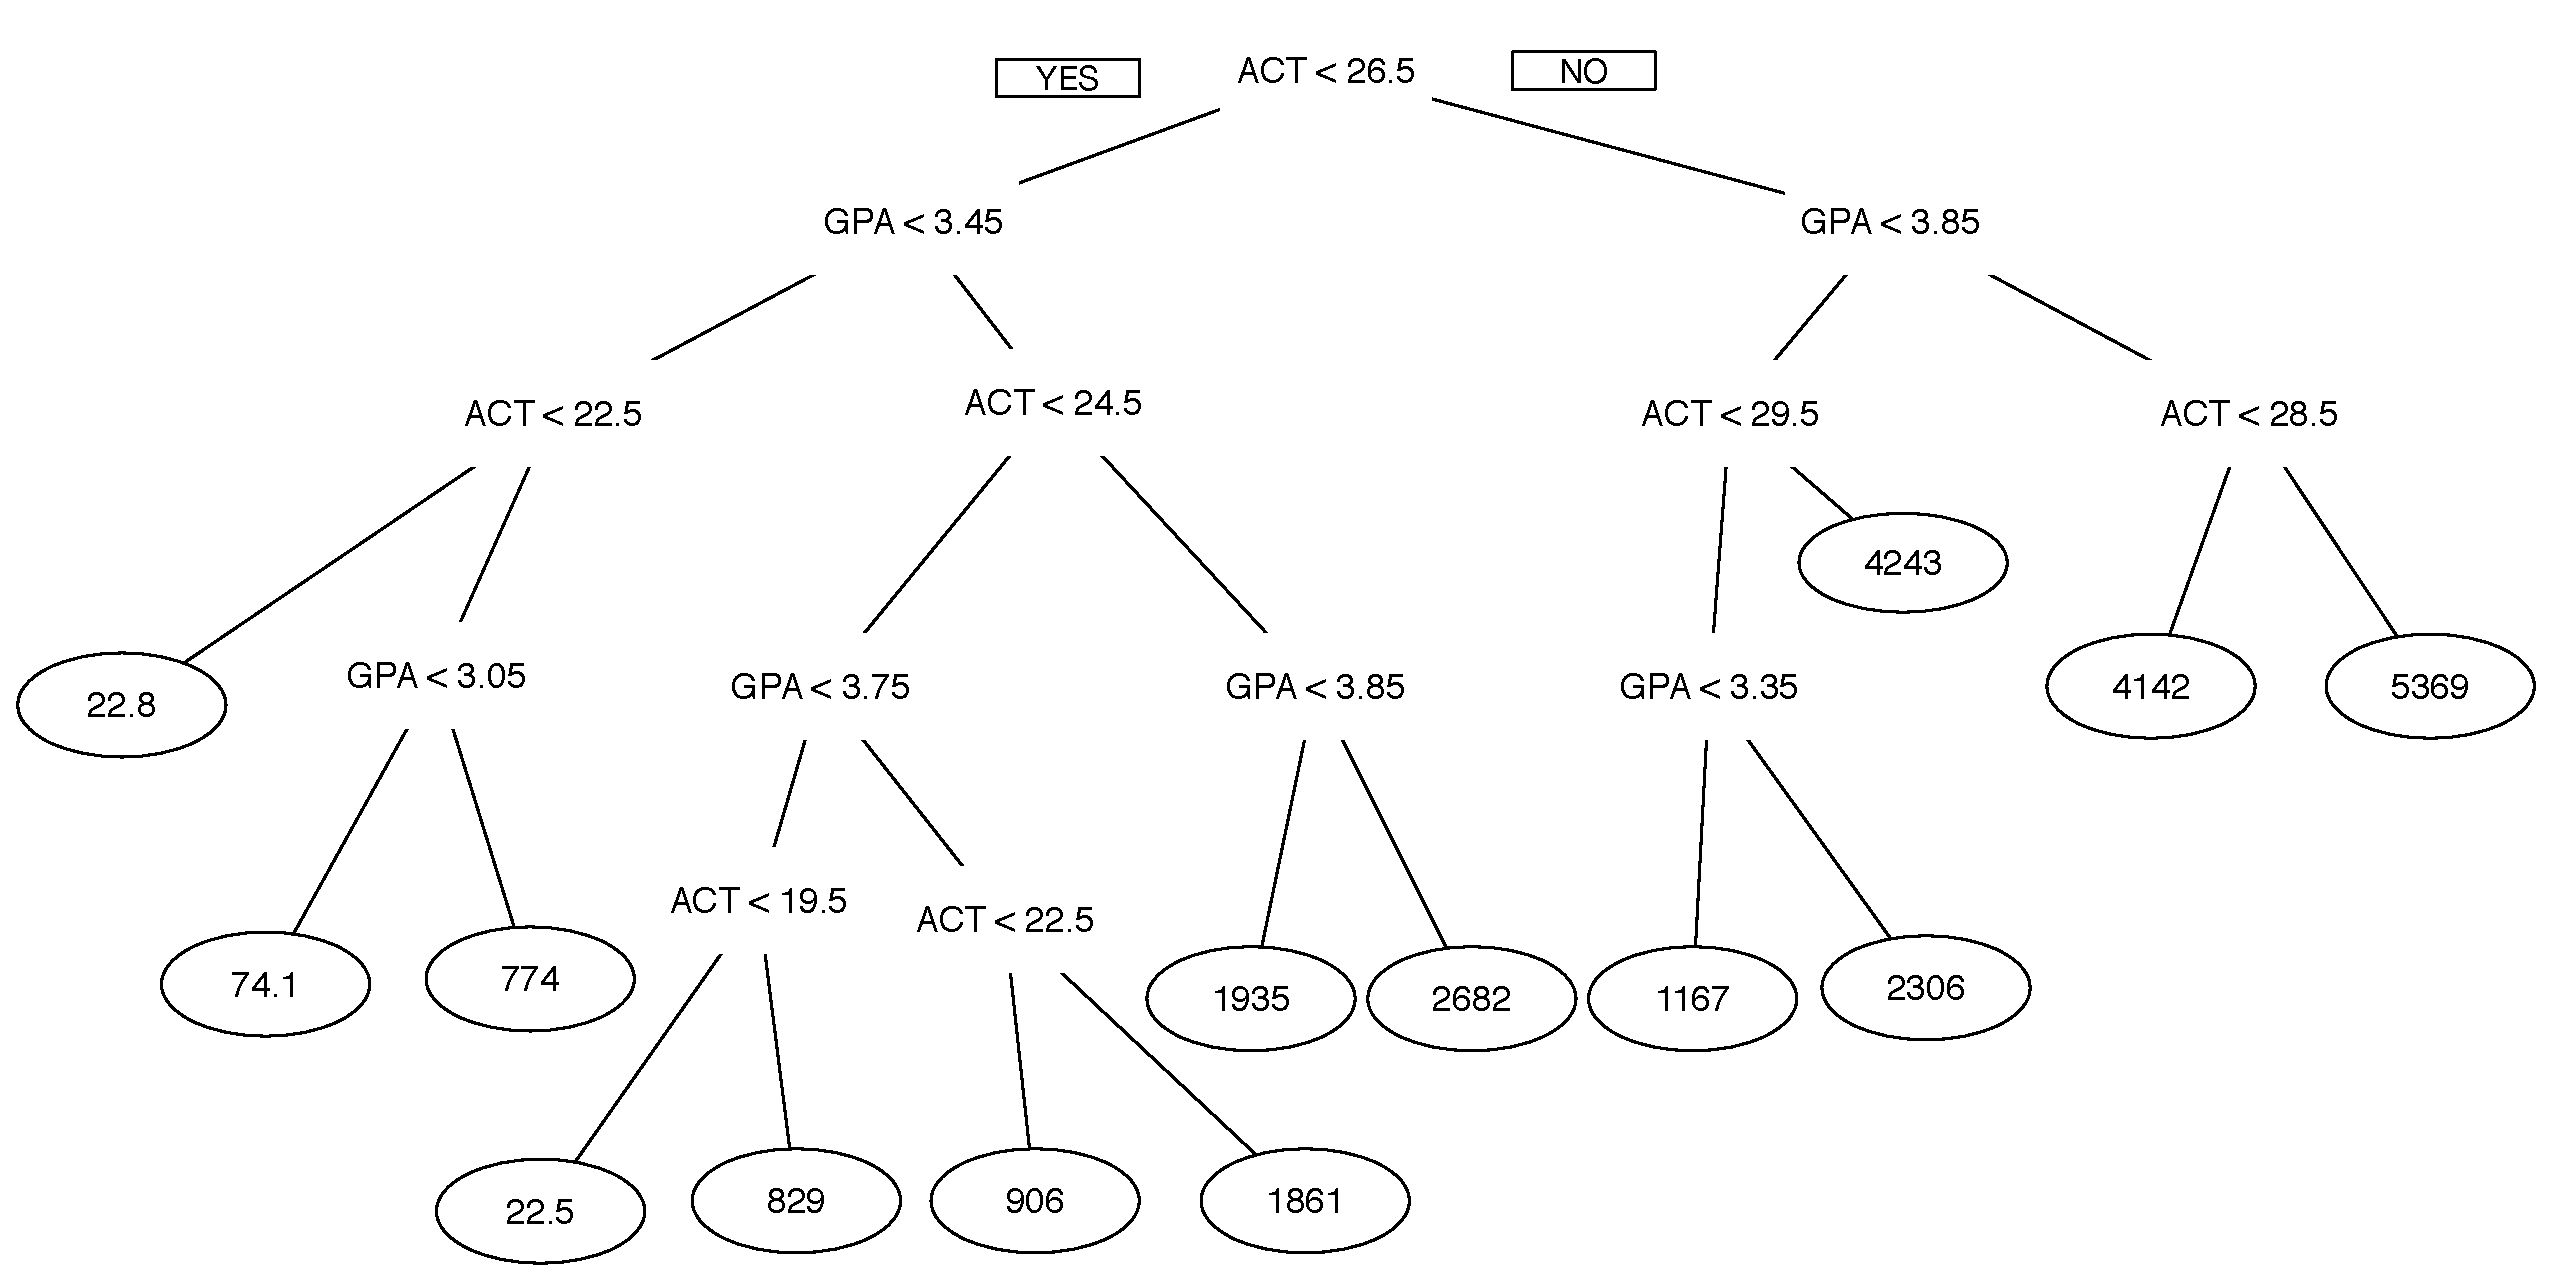
\includegraphics[width=10cm, height=6cm, scale = 0.4]
{pic/FA_DT_Result.eps}  
\end{center}
\end{frame}




\begin{frame}
\begin{centering}
\frametitle{Optimization Mean Scholarship vs GPA and ACT}
  \includegraphics[width=13.5cm, height=7cm, scale = 0.4]{pic/gpa_act.png}
  \end{centering}
\end{frame}


\begin{frame}
\frametitle{Piecewise linear regression based policy}

Piecewise linear regression using composite score:
\begin{table}[H]
\centering
\begin{tabular}{|c|c|c|}
\hline
Composite Score & \# of Applicants & Scholarship Amount \\ \hline
0-53.9         & 2,897  &0              \\ \hline
54-68.9        & 2,103  &$309\times CS -16,380 $            \\ \hline
69-76.9        &  241 &  $101\times CS - 2,024$           \\ \hline
77-80       & 19 &   $711 \times CS -48,910$          \\ \hline
\end{tabular}

\end{table}
\end{frame}




\begin{frame}
\frametitle{Piecewise linear regression based policy}
Simplified version of policy in piecewise regression form.
\begin{table}[H]
\centering
\begin{tabular}{|c|c|c|} \hline
Composite Score & Scholarship Amount & \# of Applicants \\ \hline
0-54.9          & 0        & 3,074       \\ \hline
55-59.9         & 1,500    & 872         \\ \hline
60-65.9         & 2,500    & 812         \\ \hline
66-69.9         & 3,500    & 298         \\ \hline
70-74.9         & 4,500    & 166          \\ \hline
75+             & 6,000    & 38         \\ \hline
\end{tabular}
\end{table}
Note: 41.6\% applicants receive scholarship.
\end{frame}


\begin{frame}
\frametitle{Business impact and Application}
\begin{itemize}
\item  The result of the study has been successfully implemented in the 
state university and has resulted in millions of financial benefits. 
\item The research would be applicable to many other institutions and 
offers a methodology, tools and insights into the solution of financial aid 
problems. 

\end{itemize}

\end{frame}


\begin{frame}
\frametitle{Business impact and Application}
  \begin{center}
    \begin{table}[H] 
%    \small %43
\centering
\begin{tabular}{|c|c|c|c|c|}
\hline
& 2013 & 2014 & \# Increase & \% Increase \\ \hline
Application                    & 6,101 & 6,068 & -43         & -0.7\%      \\
\hline
Admitted                       & 4,541 & 4,773 & 232         & 5.1\%       \\
\hline
Non-Scholarship                & 2,166 & 2,157 & -9          & -0.4\%      \\
\hline
Scholarship Award              & 2,375 & 2,616 & 241     & \textbf{10.1\% }

\\
\hline
%\% of scholarship              & 52\% & 55\% &             &             \\
%\hline
Matriculated                   & 2,001 & 2,222 & 221         & \textbf{11.0\%} 

\\
\hline
%Non-Scholarship Student        & 931  & 1000 & 69          & 7.4\%
%\\\hline
%Scholarship Student            & 1070 & 1222 & 152         & 14.2\%
%\\\hline
%Scholarship Matriculation Rate & 45\% & 47\% &             &             \\
\end{tabular}
\end{table}
  \end{center}
\end{frame}




\begin{frame}
  \frametitle{Business impact and Application}
  \includegraphics[width=13cm, height=7cm, scale = 0.4]{pic/results.png}

\end{frame}


\subsection{Summary}
\begin{frame}
\frametitle{Summary}
\begin{enumerate}
\item A series of models are developed to predict:
  \begin{itemize}
    \item Enrollment probability
    \item Graduation probability
    \item Number of years of stay
  \end{itemize}
\item Developed minimum cardinality dominance table to reduce the model size. 
\item An optimization model is developed with the objective to maximize the
revenue.
\item A regression analysis is developed to translate the optimization 
results to managerial insights and derive a policy for implementation.
\end{enumerate}
\end{frame}






\subsection{Limitation}
\begin{frame}
\frametitle{Limitation}
\begin{enumerate}

\item The prediction of student's enrollment decision is hard.
\item The research is also limited by the availability of 
data provided by the institution under study.
\end{enumerate}

\note[item]{is by itself a hard problem, because 
enrollment in a particular institution is determined by 
many factors that are not available to the institution.
For example, it is well known that the students' decision  is affected by
family influence and other factors, which are not traceable or measurable.}

\note[item]{Data limitaion, the quliaty and quantity of the data we have is not
very ideal, there are lots of missing information, which limits the
performance of the predction}
\end{frame}

\subsection{Future Study}
\begin{frame}
\frametitle{Future Study}
The results from the optimization specify the scholarship awards to 
each applicant under a specific population and budget.  
\begin{itemize}
\item  The actual size and composition of the application pool could be
affected by the
       unemployment rate and is random in nature. 
%\item  Stochastic optimization techniques such as sampling to find 
%the optimal allocation under a random pool will be of great 
%interest. 

\item Uncertainty: Budget, SSI, etc,. Use scenario analysis.

\end{itemize}

\note[item]{Nevertheless, at this stage, this study is on optimization under a
specific pool}
\end{frame}




\section{Acknowledgement}
\begin{frame}
  \frametitle{Thank you!}
    Dissertation Committee:
    \begin{itemize}
    \item Dr. Xinhui Zhang
    \item Dr. Pratik Parikh
    \item Dr. Caroline Cao
    \item Dr. Subhashini Ganapathy
    \item Dr. Nan Kong
    \end{itemize}
\note{ I would like to express my sincere gratitude to my advisor DR. Zhang for
the continuous support of my study. 
    Thank you for your patience, motivation and knowledge.}
\note{Besides my advisor, I would like to thank the rest of my 
thesis committeei DR......  for serving  my committee.
I want to thank you for letting my defense be an
enjoyable moment, 
and thank you for the invaluable comments and
suggestions, thanks 
to   you.}
\end{frame}




\begin{frame}
\frametitle{Backup}
\framesubtitle{Stochastic Boosting}
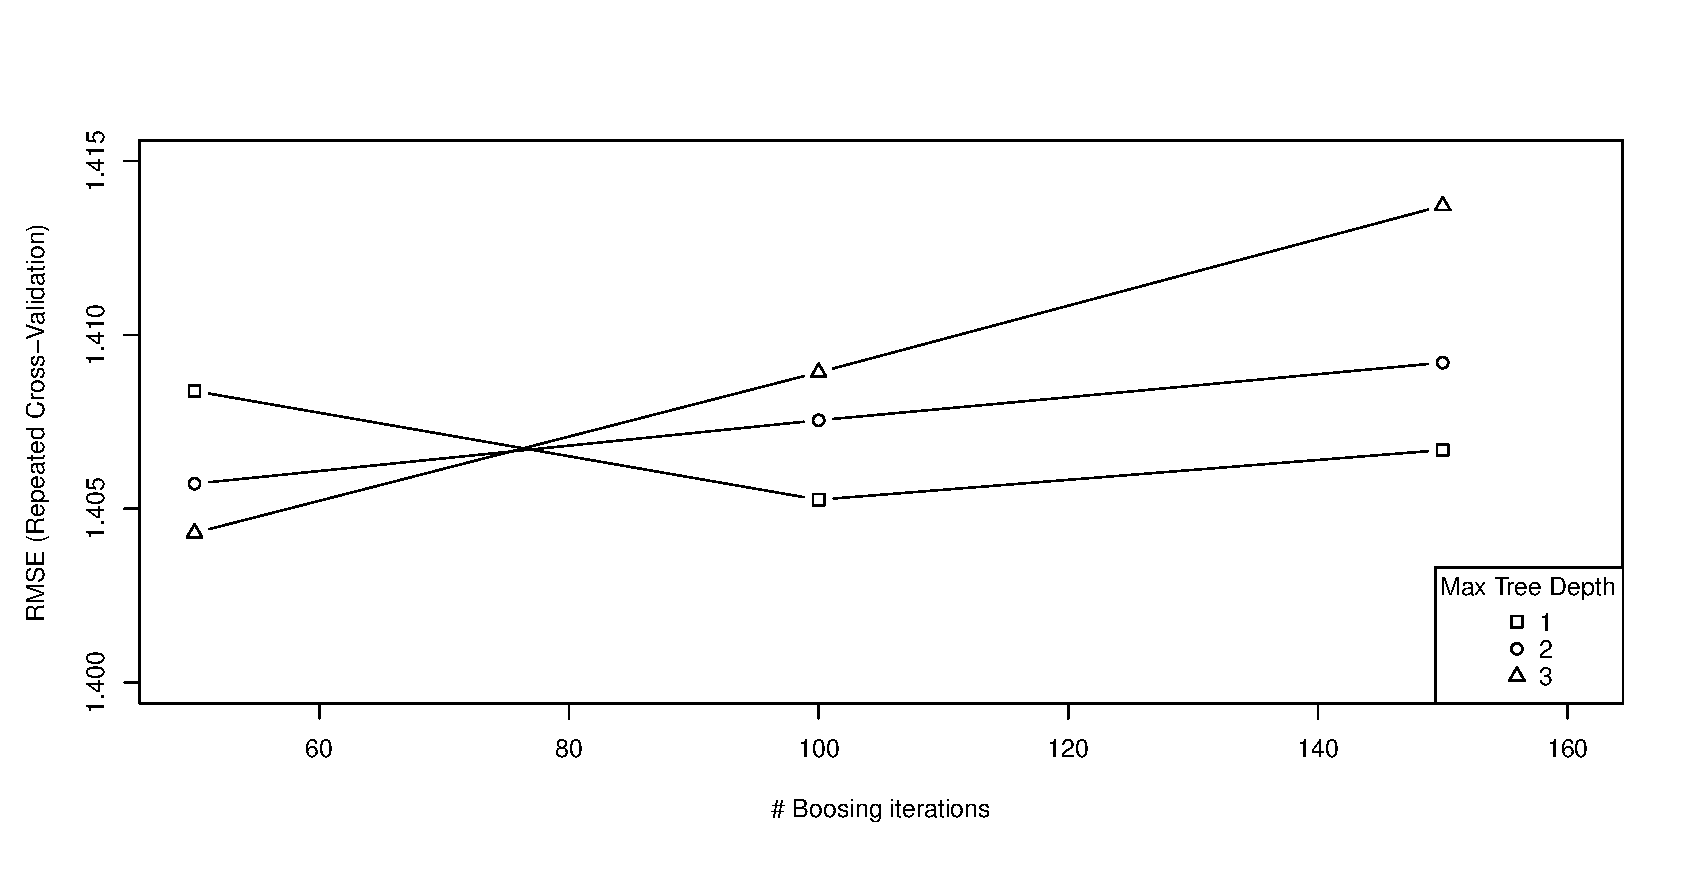
\includegraphics[width=13cm, height=7cm, scale = 0.5]
{pic/Stochastic_boositing.eps}
\end{frame}


\begin{frame}
\frametitle{Backup}
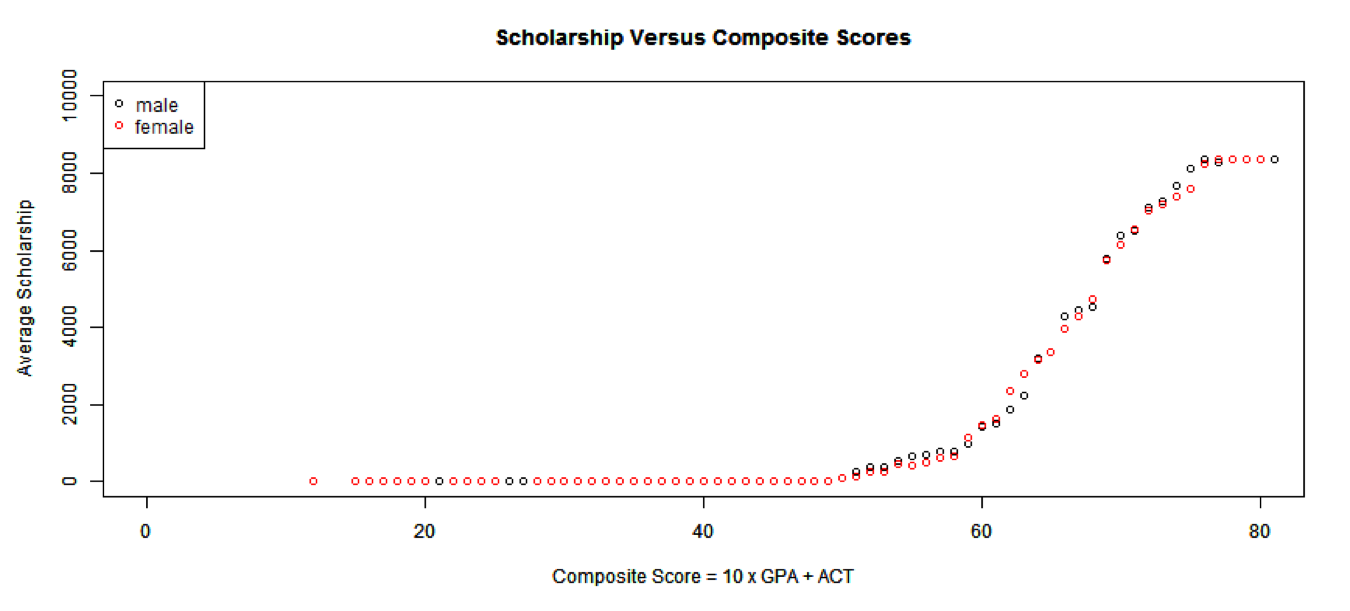
\includegraphics[width=13cm, height=7cm, scale = 0.5]
{pic/gender.png}
\end{frame}



\begin{frame}
\frametitle{}
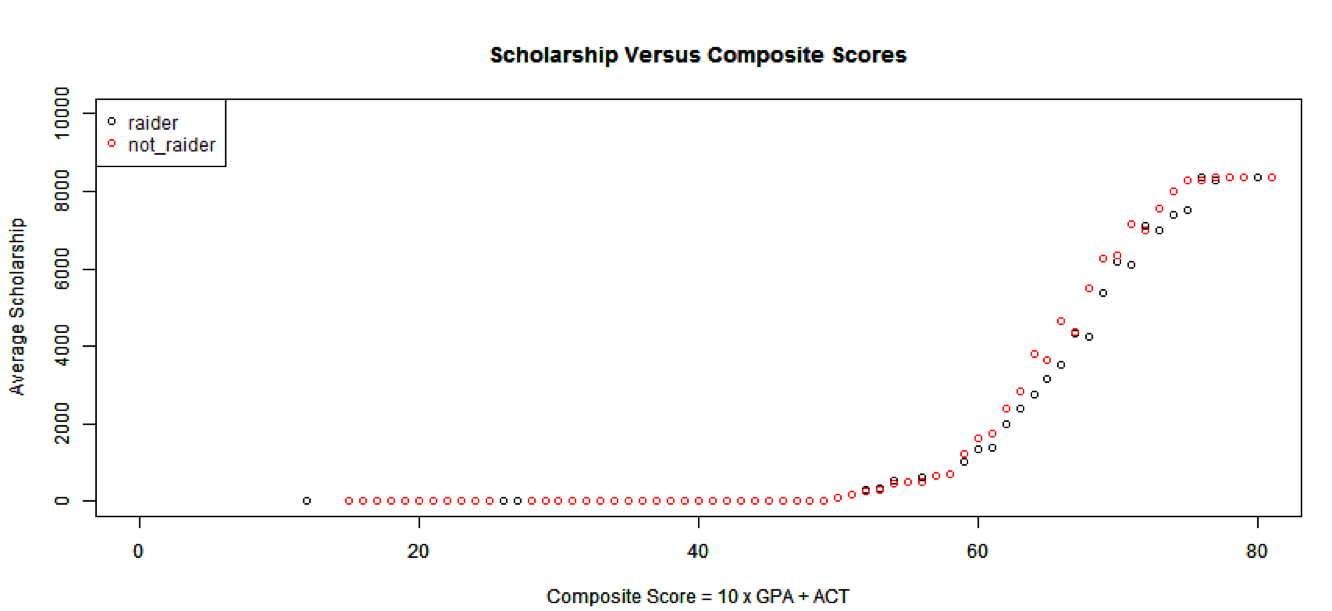
\includegraphics[width=13cm, height=7cm, scale = 0.5]
{pic/Raider.png}
\end{frame}


\begin{frame}
\frametitle{}
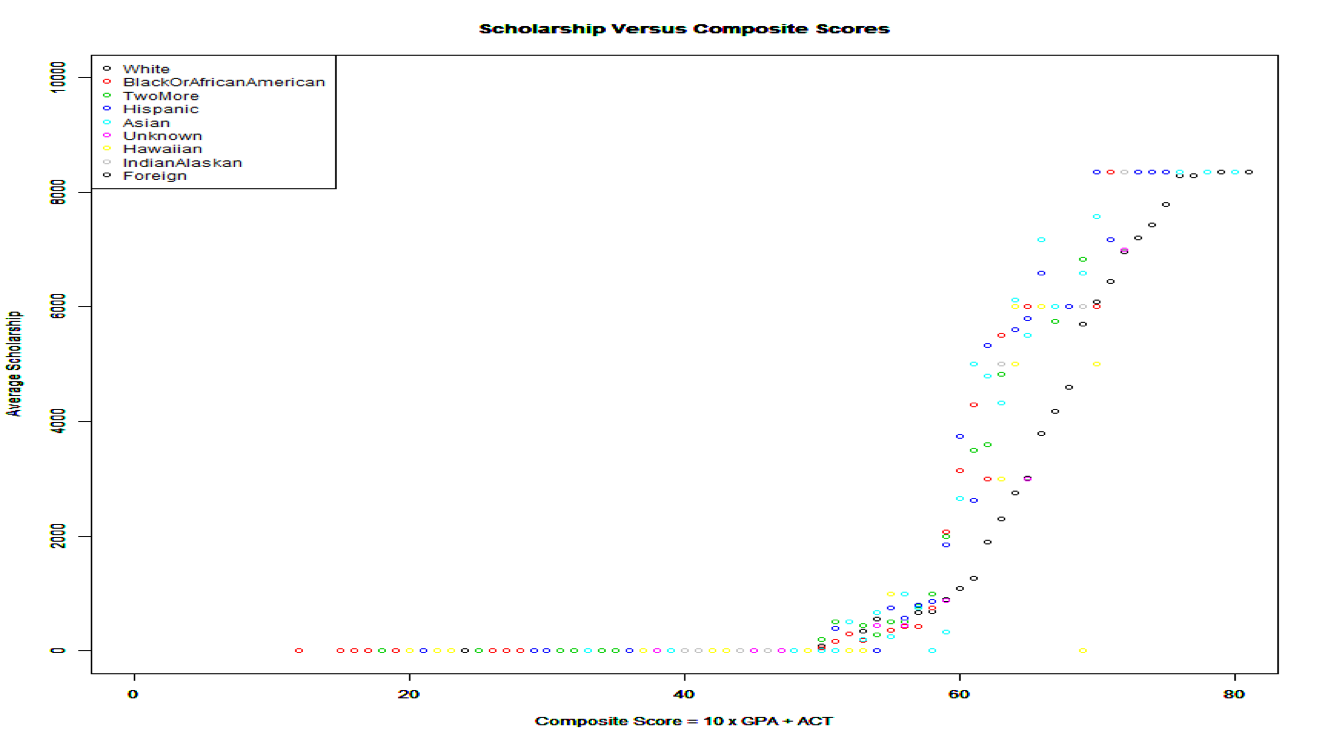
\includegraphics[width=13cm, height=7cm, scale = 0.5]
{pic/ethnicity.png}
\end{frame}



\begin{frame}
\frametitle{}
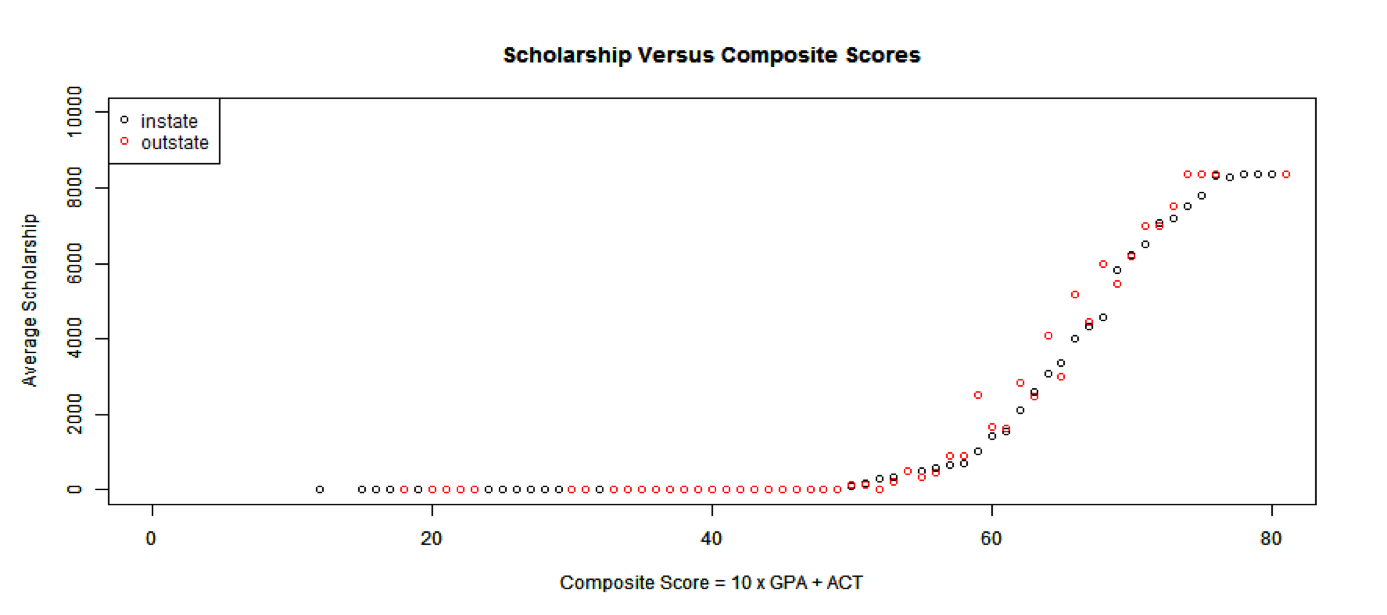
\includegraphics[width=13cm, height=7cm, scale = 0.5]
{pic/state.png}
\end{frame}


\begin{frame}
\frametitle{What is the SSI formula?}

SSI dollars are distributed directly to Ohio's public colleges 
and universities through a formula primarily driven by enrollments that 
are classified into models based on levels of instruction and the 
statewide average costs of each model. For example, it costs more for a 
campus to offer an advanced engineering course than it costs to offer an
introductory history course. Therefore, enrollments in introductory 
courses are funded at a lower rate than enrollments in more advanced 
courses.

Source: https://www.ohiohighered.org/board-of-regents/legislative-
services/faq
\end{frame}



\begin{frame}
    \frametitle{Logistic Regression}
Logistic regression generates the coefficients of a formula to predict a
logit 
transformation of the probability of the binary outcome:
 
 \begin{equation}
	p(1 \mid x)=\beta_0+\beta_1 x_1+\beta_2 x_2 +\ldots+\beta_k x_k
\end{equation}
where p is the probability of the binary outcome of interests.
\end{frame}

\begin{frame}
    \frametitle{Logistic Regression}
  The logit transformation is defined as the logged odds:
  
\begin{equation}
	Odds(p) = \frac{p}{1-p} = \frac{\text{Prob of yes}}
    {\text{Prob of no}}
\end{equation}

And 
\begin{equation}
log\_xodds(p) = \ln{\frac{p}{1-p}}
\end{equation}


\end{frame}


\begin{frame}
\frametitle{odds and log odds}
  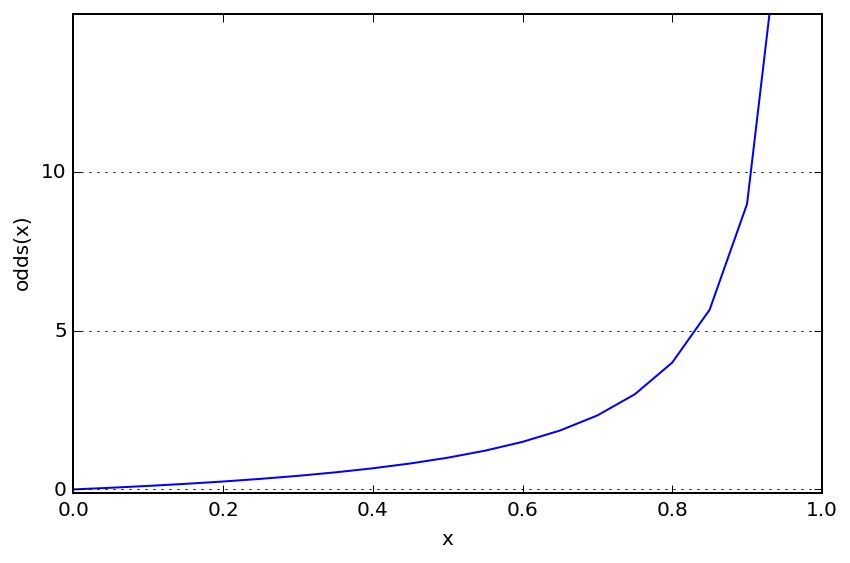
\includegraphics[scale = 0.4]{pic/odds.png}
  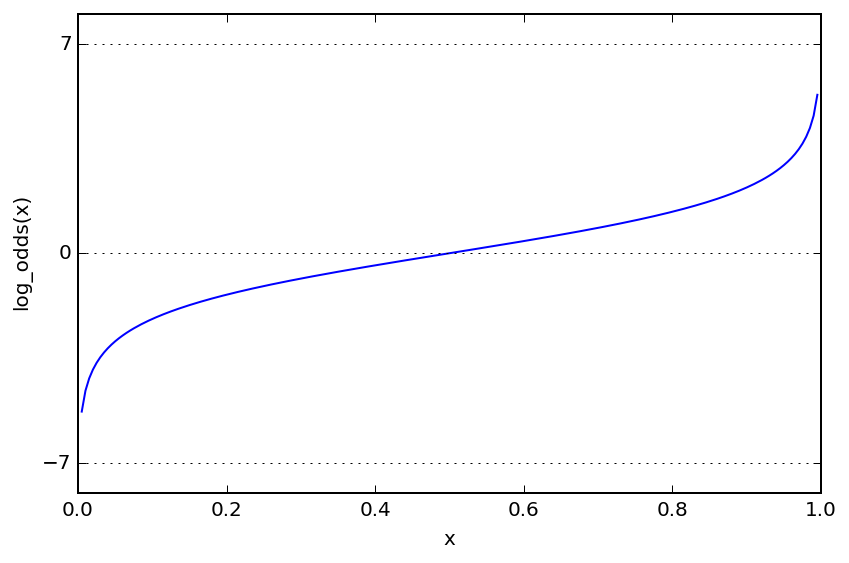
\includegraphics[scale = 0.4]{pic/logodds.png}
\end{frame}

\begin{frame}
\frametitle{Sigmoid}
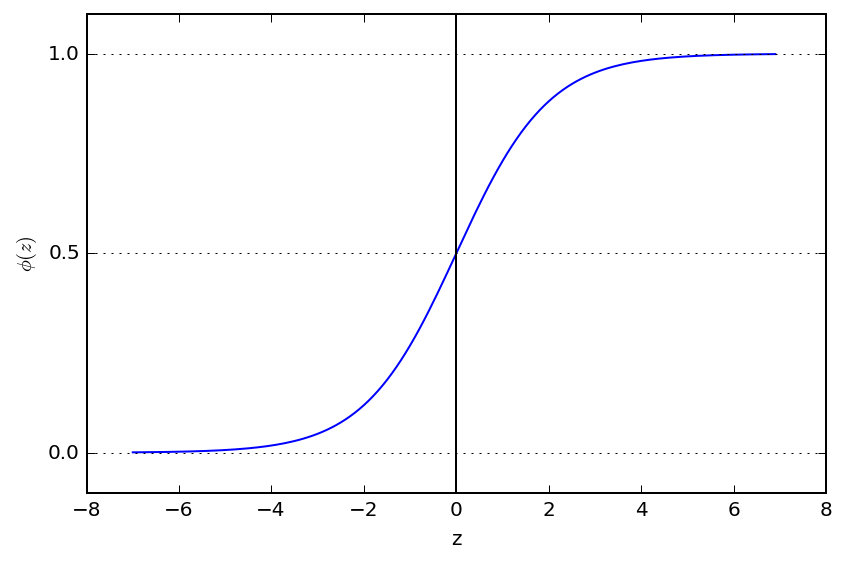
\includegraphics[scale = 0.5]{pic/sigmoid.png}  

${log\_odds}(P(y=1 \mid x)) = w_o + w_1x_1 + w_2x_2 + ... + w_nx_n$

$P(y=1 \mid x) = \phi(z) = \dfrac{1}{1 + e^{-z}}$

\end{frame}



\bibliographystyle{plainnat}
\bibliography{shuai_cita}
\end{document}



